\section{Μέθοδοι Αποτύπωσης 3D γραφικών σε εικόνα}
\label{section:rendering}
\par 
    Όταν γίνεται λόγος για μεθόδους αποτύπωσης γραφικών αναφερόμαστε στο σύστημα που συνολικά συνθέτει την τρισδιάστατη σκηνή έχοντας ως δεδομένα τις μαθηματικές αναπαραστάσεις των γεωμετρικών οντοτήτων \enit{(objects)} στο χώρο. Μετέπειτα η μηχανή γραφικών αναλαμβάνει την προβολή της σκηνής στο δισδιάστατο επίπεδο ανάλογα με το μοντέλο προβολής που έχει επιλεχθεί.
\par
    Βέβαια, αυτή η ερμηνεία του συστήματος απόδοσης δεν είναι δόκιμη. Η αποτύπωση γραφικών σε εικόνα αποτελεί, ουσιαστικά, τον τρόπο υπολογισμού του χρώματος των επιφανειών των στοιχειωδών αναπαραστάσεων, που δομούν τις επιφάνειες, με βάση το μοντέλο εικονικού φωτισμού και το μοντέλο σκίασης που ακολουθείται. Κυρίαρχο ρόλο σε αυτό παίζει η τεχνική που ακολουθείται στο κομμάτι υπολογισμού το χρώματος των εικονοστοιχείων με βάση το μοντέλο φωτισμού που ακολουθείται (είδος υλικού, είδη φωτισμού). Πάνω σε αυτό το κομμάτι υπάρχουν και φωτορεαλιστικές προσεγγίσεις του προβλήματος(πχ. ολικός φωτισμός με χρήση ιχνηλάτισης ακτίνων).
\par
    Αναφορικά στις κατηγορίες των μεθόδων σκίασης ανήκουν οι αλγόριθμοι \enit{Lambert} ή \enit{Flat Shading} και \enit{Gouraud} ή \enit{Smooth Shading}. Στο κομμάτι της προσομοίωσης του φωτισμού χωρίς φωτορεαλιστικά αποτελέσματα ανήκουν μέθοδοι όπως ο αυτοφωτισμός, ο φωτισμός διάχυσης, ο κατοπτρικός φωτισμός και το μοντέλο Phong κατοπτρικής ανάκλασης, κλασσικά τεχνάσματα φωτισμού που αποδίδουν και διαφορετικές υφές υλικών \textit{(Βασικά Μοντέλα Φωτισμού Κεφ.17 στο \cite{hearn2011computer})}. Όλα αυτά τα μοντέλα φωτισμού έχουν πρόβλημα στον υπολογισμό των σκιών οι οποίες δεν υπολογίζονται αυτόματα από το σύστημα αλλά επίσης θα πρέπει τα γραφικά να είναι άμεσα ορισμένα που σημαίνει στοιχεία που προκύπτουν από αλληλεπιδράσεις του φωτός με τα αντικείμενα θα πρέπει να είναι τεχνητά φτιαγμένα. Συνεπώς, τέτοιες πρακτικές δεν αρκούν στην ανακατασκευή γραφικών που όταν αποτυπώνονται σε εικόνες προσεγγίζουν πραγματικές φωτογραφίες. 
\par
    Εκτός από το κομμάτι του χρώματος, για να γίνει και γεωμετρική βελτίωση του μοντέλου χρειάζεται αντίστροφη αποτύπωση, δηλαδή μετάβαση από την εικόνα στον τρισδιάστατο χώρο και εύρεση των ακτίνων φωτός που πέφτουν πάνω στην επιφάνεια.Τέλος, οι οντότητες μια σκηνής προφανώς θα πρέπει να μπορούν να περιγραφούν και με έμμεσο τρόπο και όχι μόνο με άμεσο τρόπο (πλέγματα πολυγώνων [\ref{section:Graphics Representations}]). 
     
\subsection{Αλγόριθμος Ιχνηλάτισης Ακτίνων | Ray Tracing}
    \begin{figure}[H]
    \centering
    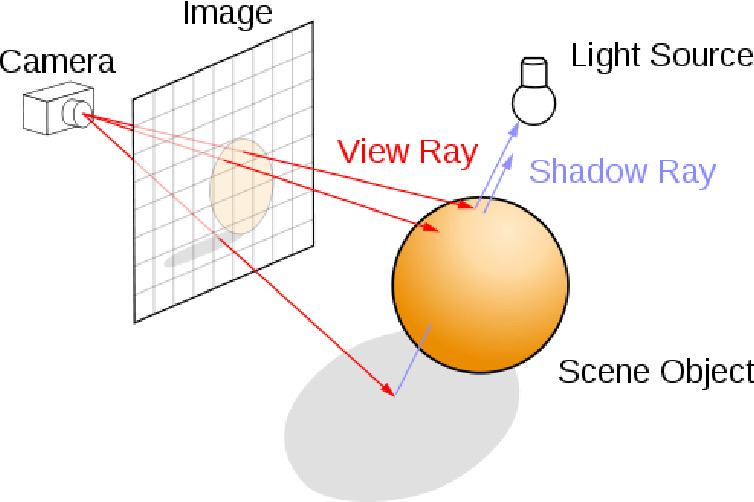
\includegraphics[width = 0.5\linewidth]{images/chapter2_img/CameraSystem.jpg}
    \caption{Σύστημα Κάμερας σε μηχανές Γραφικών που εκτελούν Ιχνηλάτιση Ακτίνας}
    \label{fig:camera system}
    \end{figure}
    Στην γραφική υπολογιστών το κομμάτι του φωτισμού, είναι μια απαιτητική και αναγκαία διαδικασία για την απόδοση χαρακτηριστικών όπως το χρώμα και η υφή του υλικού το οποίο απεικονίζεται στην σκηνή. 
    Η πορεία του φωτός παίζει εξίσου σημαντικό ρόλο εδώ, καθώς πέραν του ότι καθορίζει την θέση των σκιών δίνει πληροφορίες για ανακλάσεις που δημιουργούνται από αλλεπάλληλες ανακλάσεις του φωτός σε αντικείμενα. 
    
    H έννοια της ρίψης ακτίνων (\enit{ray casting}) χρησιμοποιείται στην δημιουργική στερεομετρία για τον εντοπισμό των τομών πάνω σε επιφάνειες, με ακτίνες που προκύπτουν από τις θέσεις των εικονοστοιχείων(UV επίπεδο βλ.Παράρτημα Κεφ.[\ref{appendix:camerasystem}]).  
    
    Ο αλγόριθμος ιχνηλάτισης ακτίνων είναι μια γενικευμένη μέθοδος ρίψης ακτίνων ως ένα μέσο εντοπισμού των ορατών επιφανειών μιας σκηνής και προτάθηκε από την επιστημονική κοινότητα όταν οι απλοί μέθοδοι φωτισμού δεν παρήγαγαν το επιθυμητό οπτικό αποτέλεσμα υπό το πρίσμα της φωτογραφικά ρεαλιστικής παραγόμενης σκηνής.
    \begin{figure}[H]
    \centering
    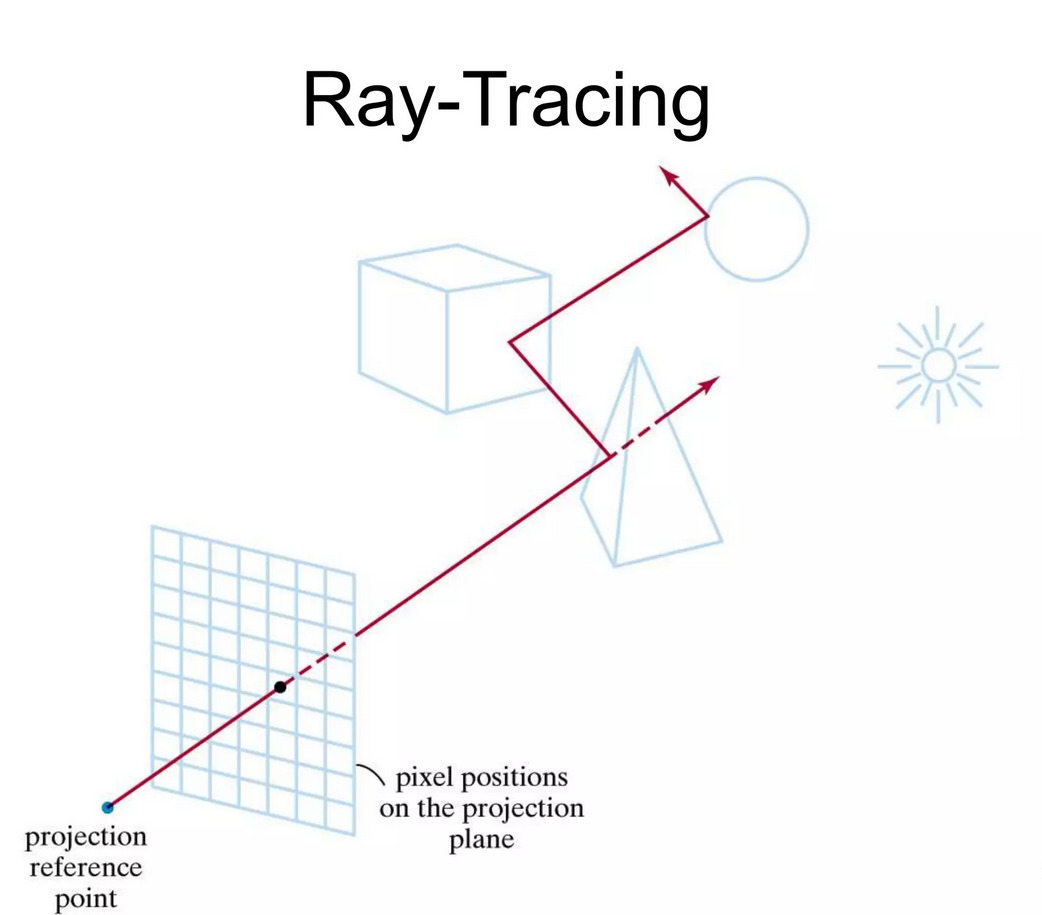
\includegraphics[width=6cm]{images/chapter2_img/ray_tracing.jpg}
    \caption{Πολλαπλά Ίχνη ανάκλασης και μετάδοσης ακτίνας που προέρχεται από το σημείο αναφοράς προβολής, περνάει μέσα από την θέση του   Πηγή:\cite{hearn2011computer}}
    \label{fig:ray-tracing-setup}
    \end{figure}
    
    Το πρόβλημα είναι πως οι πηγές δεν είναι σημειακές αλλά και επίσης τα σώματα δεν επηρεάζονται αποκλειστικά και μόνο από το φως που προκύπτει από την πηγή φωτός αλλά και από τις αλληλεπιδράσεις και τις ανακλάσεις που κάνει το φως με άλλα σώματα στην σκηνή. Έτσι, αντί απλά να ψάχνεται μια θέση ενός εικονοστοιχείου για την ορατή επιφάνεια, συνεχίζουμε την πορεία της ακτίνας που περνά από ένα εικονοστοιχείο για να γίνει συλλογή εντάσεων ακτινοβολίας από διάφορες ανακλάσεις στις επιφάνειες που περιλαμβάνει η τρισδιάστατη σκηνή. 
    
    
    Συνεπώς, αν θα μπορούσαμε να οριοθετήσουμε τον αλγόριθμο \enit{Ray Tracing} σε μια διαδικασία που απεικονίζεται με διάγραμμα ροής και βασίζεται στις παραπάνω εικόνες θα ήταν η εξής:
    \begin{figure}[H]
        \centering
        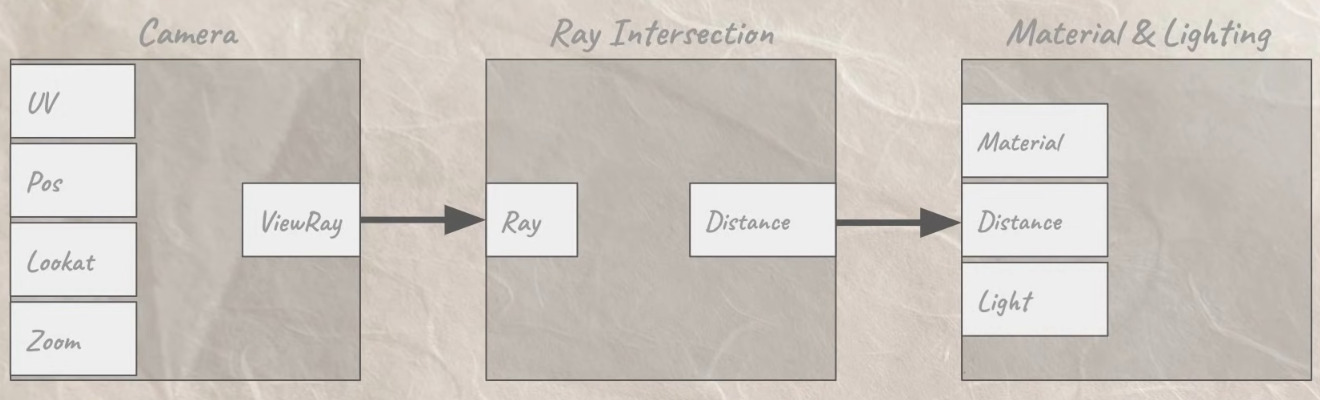
\includegraphics[width=.6\linewidth]{images/chapter2_img/ray_tracing_pipline.jpg}
        \caption{Το διάγραμμα ροής του \enit{Ray Tracing} Πηγή: \href{https://youtu.be/PGtv-dBi2wE?si=aUpxw89M65hnv-su}{Ray Marching Video}}
        \label{fig:ray_tracing_pipeline}
    \end{figure}
\par 
    Το πιο απαιτητικό κομμάτι στο διάγραμμα που καθορίζει και την γεωμετρική λεπτομέρεια που αποδίδεται στην εικόνα (και είναι αλληλένδετο με την γεωμετρική λεπτομέρεια που υπάρχει στην \enit{3D} πληροφορία), είναι το \enit{Ray Intersection}(υπολογισμός των σημείων τομής της ακτίνας με την επιφάνεια). Σε αυτό το τμήμα, έχουν βοηθήσει αρκετά νέοι αλγόριθμοι ιχνηλάτισης ακτίνας, ιδιαιτέρως σε έμμεσες αναπαραστάσεις επιφανειών με χρήση πεδίων απόστασης. 
%% Volumetric Rendering Methods - Ray marching
\subsection{Απόδοση Όγκου \\ \large {Αλγόριθμος Βηματισμού Πάνω στην Ακτίνα | Ray Marching} }
\par
    O αλγόριθμος ιχνηλάτισης ακτίνας, υπολογίζει επακριβώς τα σημεία τομής της επιφάνειας με την ακτίνα που πάνω στην κατεύθυνση προβολής. Αυτό μπορεί να αποβεί μοιραίο υπολογιστικά, ιδιαιτέρως όταν η γεωμετρία που αναπαριστάται είναι αρκετά σύνθετη και δεν περιγράφεται άμεσα. Για αυτόν τον λόγο οι κλασσικές μέθοδοι ιχνηλάτισης ακτίνας δεν χρησιμοποιούνται στην απόδοση ογκομετρικών γραφικών. 
\par
    Μια πιο συνετή επιλογή είναι ο Αλγόριθμος Βαδίσματος πάνω στην ακτίνα, \enit{Ray Marching}, που σκοπό δεν έχει να βρει το ακριβές σημείο πάνω στην επιφάνεια αλλά να κάνει βήματα από την αρχή της ακτίνας προς την επιφάνεια και να φτάσει όσο τον δυνατόν πιο κοντά στην επιφάνεια. Αποτέλεσμα αυτού, πρώτον ότι δεν είναι απαραίτητοι όλοι οι υπολογισμοί που κάνει το \enit{Ray Tracing} και δεύτερον η αξιοπιστία των αποτελεσμάτων παραμένει υψηλή. Τέλος μετασχηματισμοί και παραμορφώσεις σε γραφικές αναπαραστάσεις δεν επιβαρύνουν την λειτουργία του αλγορίθμου (ο οποίος ψάχνει σημεία τομής), ενώ αντιθέτως στο \enit{Ray Tracing} αυτό αποτελεί τροχοπέδη, για αυτό συνήθως ο τελευταίος χρησιμοποιείται για στατικά γραφικά απλής γεωμετρίας που συνήθως ορίζονται άμεσα.
\par
    Επί του πρακτέου, χρησιμοποιείται ο αλγόριθμος βαδίσματος πάνω στην ακτίνα ο οποίος αποτελεί εκ φύσεως, έναν άπληστο αλγόριθμο αφού ψάχνει τον χώρο για τομή με επιφάνειες. Έτσι, για την εφαρμογή του γίνεται μια σειρά πεπερασμένων βημάτων κατά την διεύθυνση της ακτίνας μέχρι να έρθει σε επαφή η ακτίνα πάνω σε κάποιο αντικείμενο της σκηνής ή να ξεπεραστεί ο αριθμός των \textbf{πεπερασμένων βημάτων} που επιλέγονται ως συνθήκη τερματισμού του αλγορίθμου\footnote{για να μη επεκτείνει την ακτίνα προς το άπειρο}. Συνεπώς μια συνοπτική αλγοριθμική παρουσίαση του αλγορίθμου περιλαμβάνει τα εξής βήματα: 
    
    \begin{algorithm}[H]
    \caption{Απλοική μορφή Ray Marching}
    \begin{algorithmic}[1]
    \State Ρίψη ακτίνας προς την 3D σκηνή μέσα από το UV επίπεδο της φωτογραφίας
    \State Αρχικοποίηση μεταβλητών
    \State Ορισμός μεγίστου αριθμού βημάτων MAX\_STEPS
    
    \For{κάθε pixel στο UV επίπεδο της φωτογραφίας}
        \State $p \gets$ αρχική θέση της ακτίνας
        \State $d \gets$ αρχική απόσταση
        \State $i \gets 0$
        \While{$i < \text{MAX\_STEPS}$ και $d > \text{MIN\_DISTANCE}$}
            \State Υπολογισμός πεδίου απόστασης $d(p)$
            \State Προώθηση της ακτίνας προς την κατεύθυνση του κοντινότερου object
            \State $i \gets i + 1$
        \EndWhile
        \State Εφαρμογή επεξεργασίας για την απόδοση του χρώματος στο pixel
    \EndFor
    \end{algorithmic}
    \end{algorithm}
    % \clearpage
    
\subsubsection{Χρήση Πεδίων Προσημασμένης Απόστασης σε συνδυασμό με τον αλγόριθμο Ray Marching - Sphere Tracing}
    \begin{figure}[H]
        \centering
        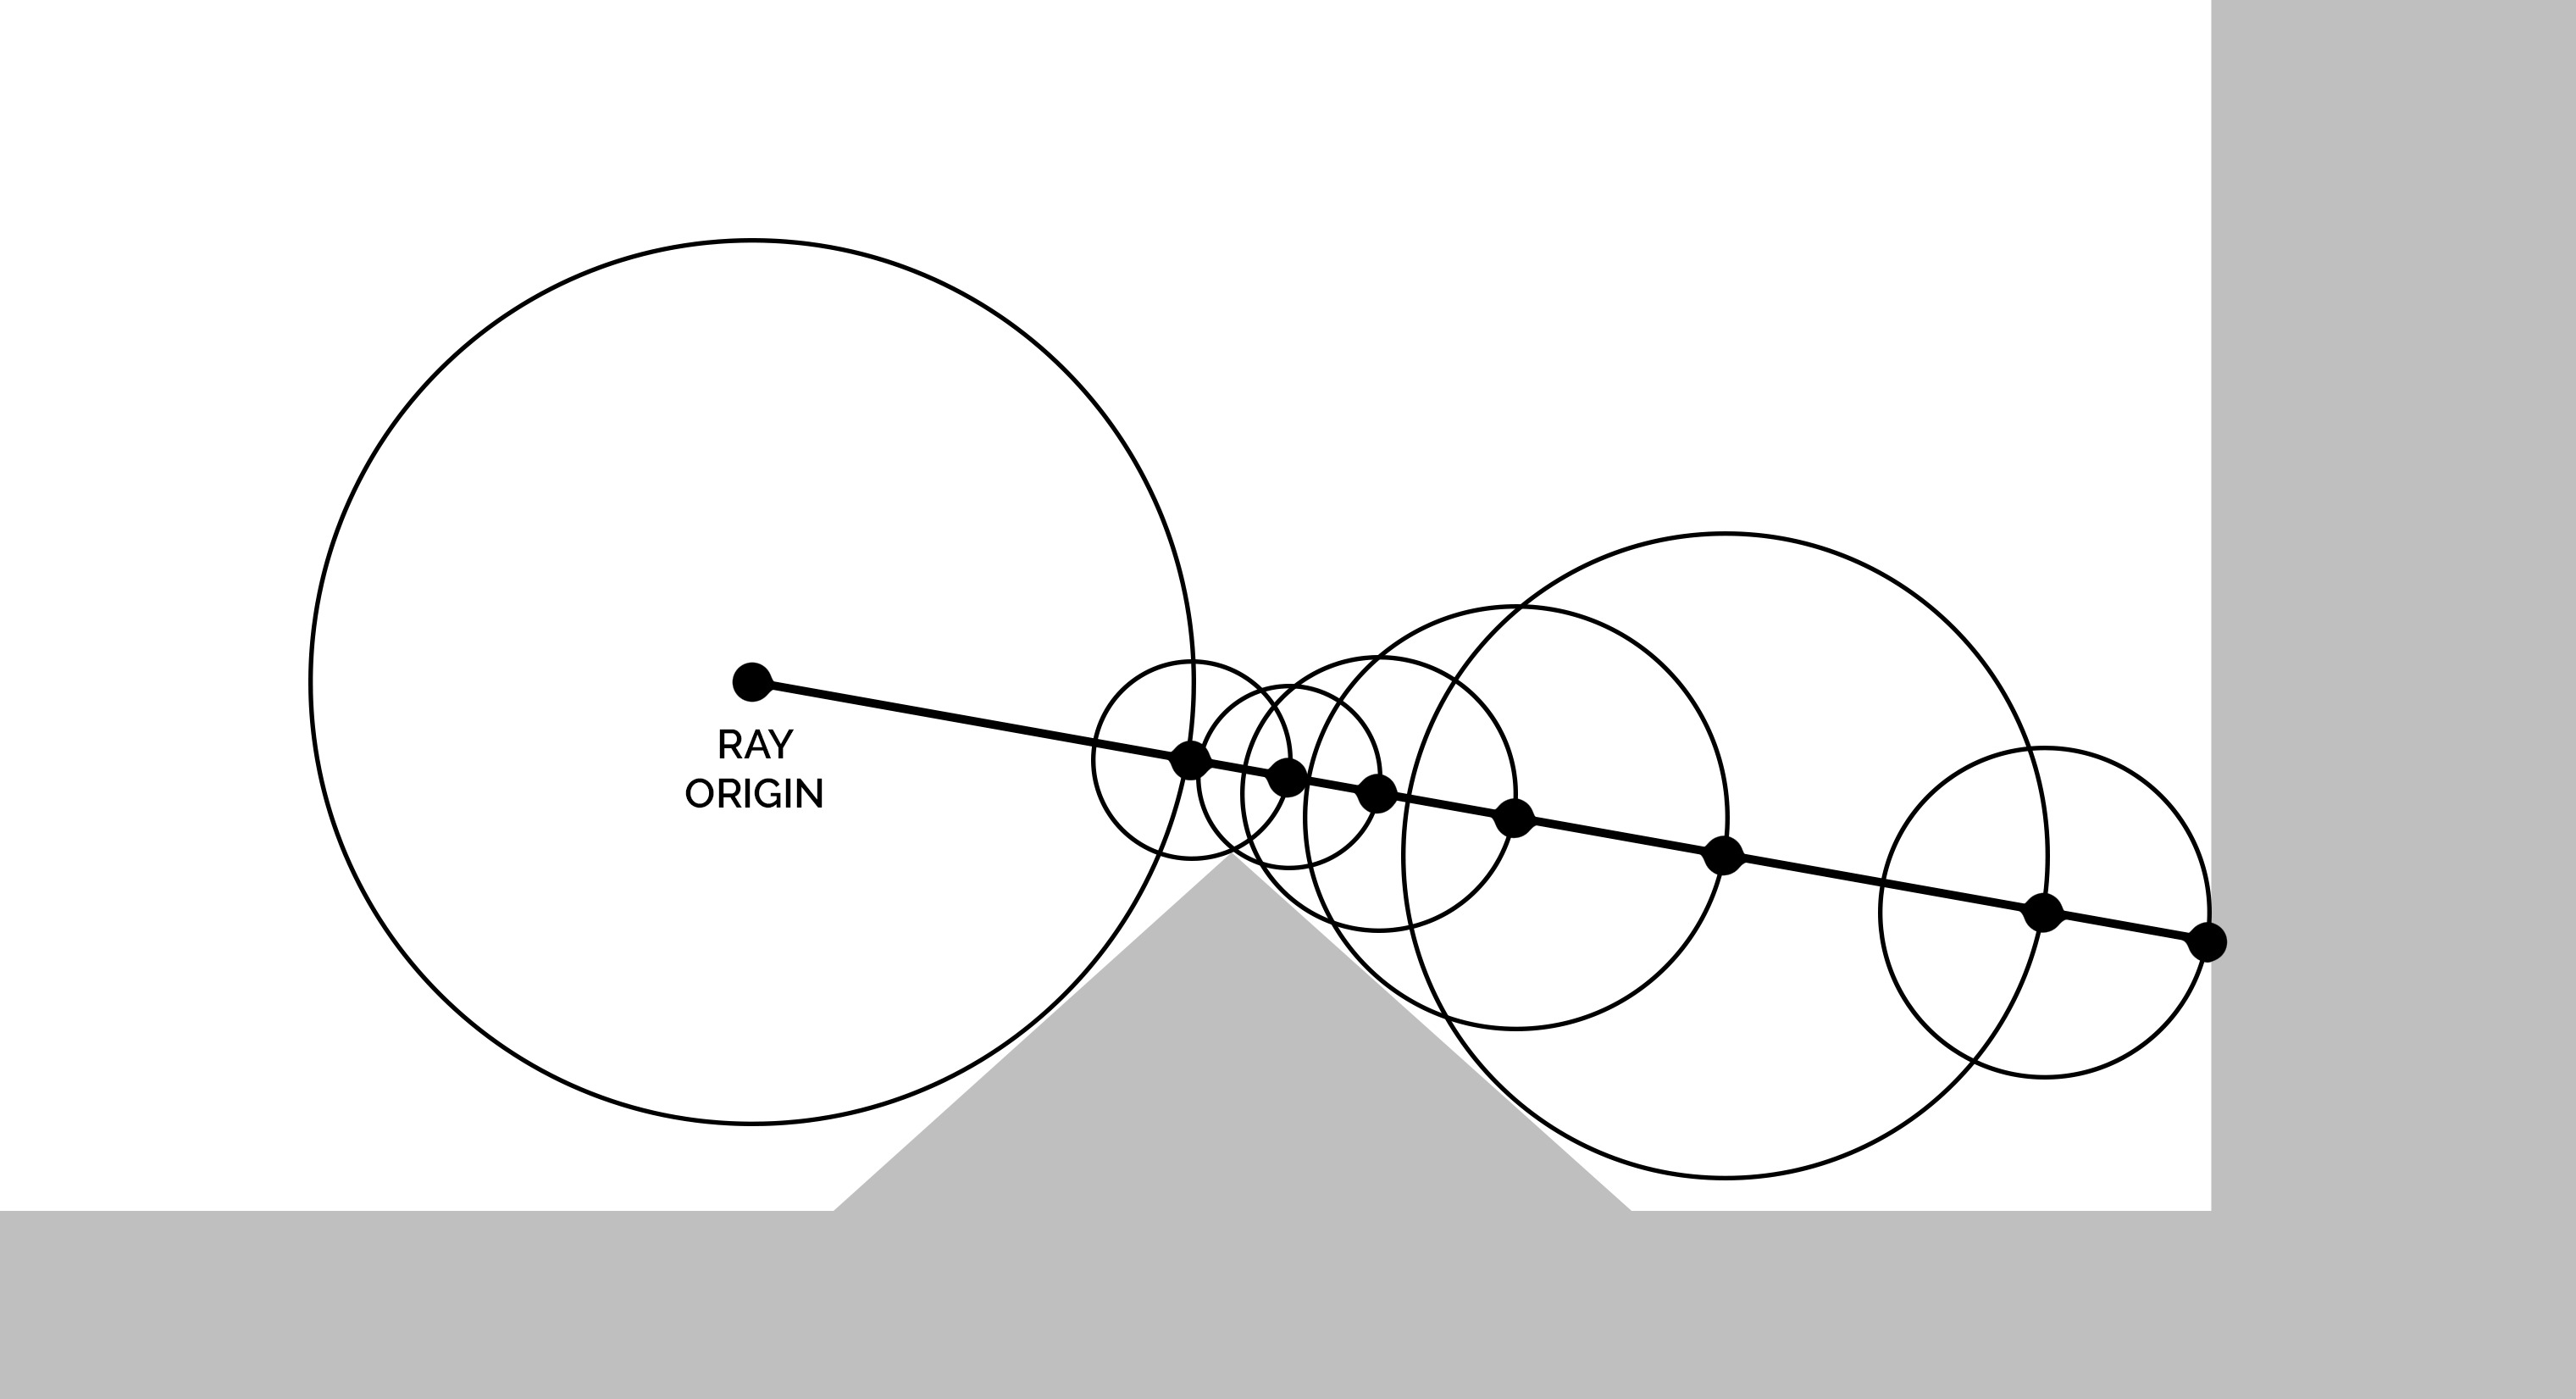
\includegraphics[width=.4\linewidth]{images/chapter2_img/Visualization_of_SDF_ray_marching_algorithm.jpg}
        \caption{\small{Χρήση Βαδίσματος Ακτίνας για την εύρεση Σημείων τομής με δομές του χώρου με χρήση σφαιρικού έλεγχου προσημασμένης απόστασης(Sphere Tracing) - 2D}}
        \label{fig:Ray Marching Vizualization Sphere Tracing}
    \end{figure}

O  John C. Hart στην αντίστοιχη εργασία του \cite{JohnHartSphereTracing} έδωσε την ιδέα υλοποίησης του αλγορίθμου, για απόδοση τρισδιάστατων σκηνών από έμμεσες επιφάνειες πολλών μορφών μεταξύ και πεδίων προσημασμένης απόστασης, όπου η επιφάνεια ορίζεται ως επιφάνεια απόστασης d=0 στην συνάρτηση προσημασμένης απόστασης και εντός της η απόσταση είναι αρνητική. 
\begin{algorithm}[H]
\caption{Sphere Tracing Algorithm}
\begin{algorithmic}
\State Initialize the ray with an initial position and direction.
\State Set the step size $t$ and maximum distance $T$.
\While{Termination condition is not met}
    \State Calculate the current position along the ray: $p = \text{initial position} + t \cdot \text{direction}$.
    \State Evaluate the implicit function at the current position: $f(p)$.
    \If{$f(p)$ is less than a predefined threshold (indicating proximity to the surface), terminate the loop.}
    \EndIf
    \State Update $t$ using a specific step size function.
\EndWhile
\State Calculate the surface normal at the intersection point.
\State Calculate the final color and shading at the intersection point for rendering.
\end{algorithmic}
\end{algorithm}
Αυτός ο αλγόριθμος είναι μια απλοϊκή μορφή του \enit{Sphere Tracing} που χρησιμοποιείται και στην παρούσα εργασία.

\subsection{Διαφορίσιμη αποτύπωση έμμεσων πεδίων  \enit{Implicit Differentiable Rendering}}
Στην παρούσα εργασία χρησιμοποιείται ο αλγορίθμος βαδίσματος πάνω στην ακτίνα \enit{Ray Marching/Sphere Tracing} μέσω του οποίου γίνεται δυνατή η εκπαίδευση της γεωμετρίας του χώρου που αναπαρίσταται. Η διαφορά έγκειται, στο ότι έχουμε ένα εκπαιδεύσιμο πεδίο προσημασμένης απόστασης το οποίο μεταβάλλεται και χρησιμοποιείται ταυτόχρονα η διαδικασία του \enit{Sphere Tracing} κατά την εκπαίδευση. Περισσότερα στο κεφάλαιο της μεθοδολογίας με την διαφορική μορφή εξίσωσης απόδοσης \ref{eq:differentiableRendering}.
\clearpage

